% Provenance (never printed): old premiere S material on the formation of fossil
% fuels (preserved organic matter, burial, oil window, migration, trap, coal).
% Burial history of the invented Merrow Basin from figdata/grade-11/oil_window.py
% (constant geotherm, no compaction). Rifts and passive margins after the USGS
% West-Central Coastal Province fact sheet (2023-3028). Folds are defined in
% g12.02 mountain-building (Sync 0): the anticline is told in prose here, never
% defined. Sedimentary basins compared, diagenesis: Year 1/2.
\chapter{煤、石油和天然气的地质学}\label{ch:g11:fossil-fuel-geology}

一块取自宾夕法尼亚一座旧煤矿的黑色页岩板上，
保存着蕨类植物样的叶片，它们在深色岩石的映衬下呈扁平的银色。
这些植物生长于三亿多年前的沼泽中，
时代为石炭纪；它们在腐烂之前即被掩埋，因而保留了原有形状，沼泽植物的碳则变成了煤。
今天从海上平台开采的石油和天然气，
与之成因相同：它们都是活着的生物留下的遗体，
这些遗体逃脱了腐败，随后被掩埋并受热。本章
将沿着这些被埋藏的碳，从沼泽和海底出发，
一直追踪到煤层和油田。
% ledger: photo:g11-fossil-plants, ics:base.Carboniferous, ics:base.Permian, earle:coal-formation, earle:organic-preservation

\begin{omfigure}
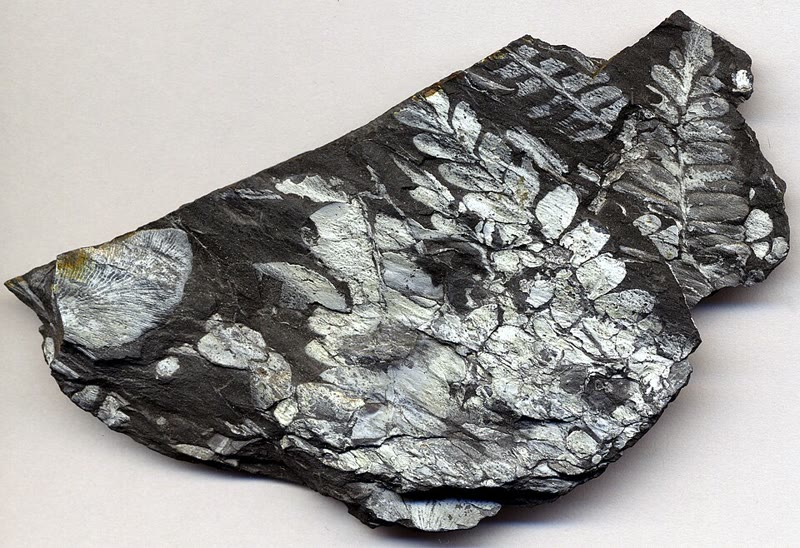
\includegraphics[height=4.4cm]{images/book2/g11-stjohn-fossil-plants.jpg}\hspace{0.03\linewidth}%
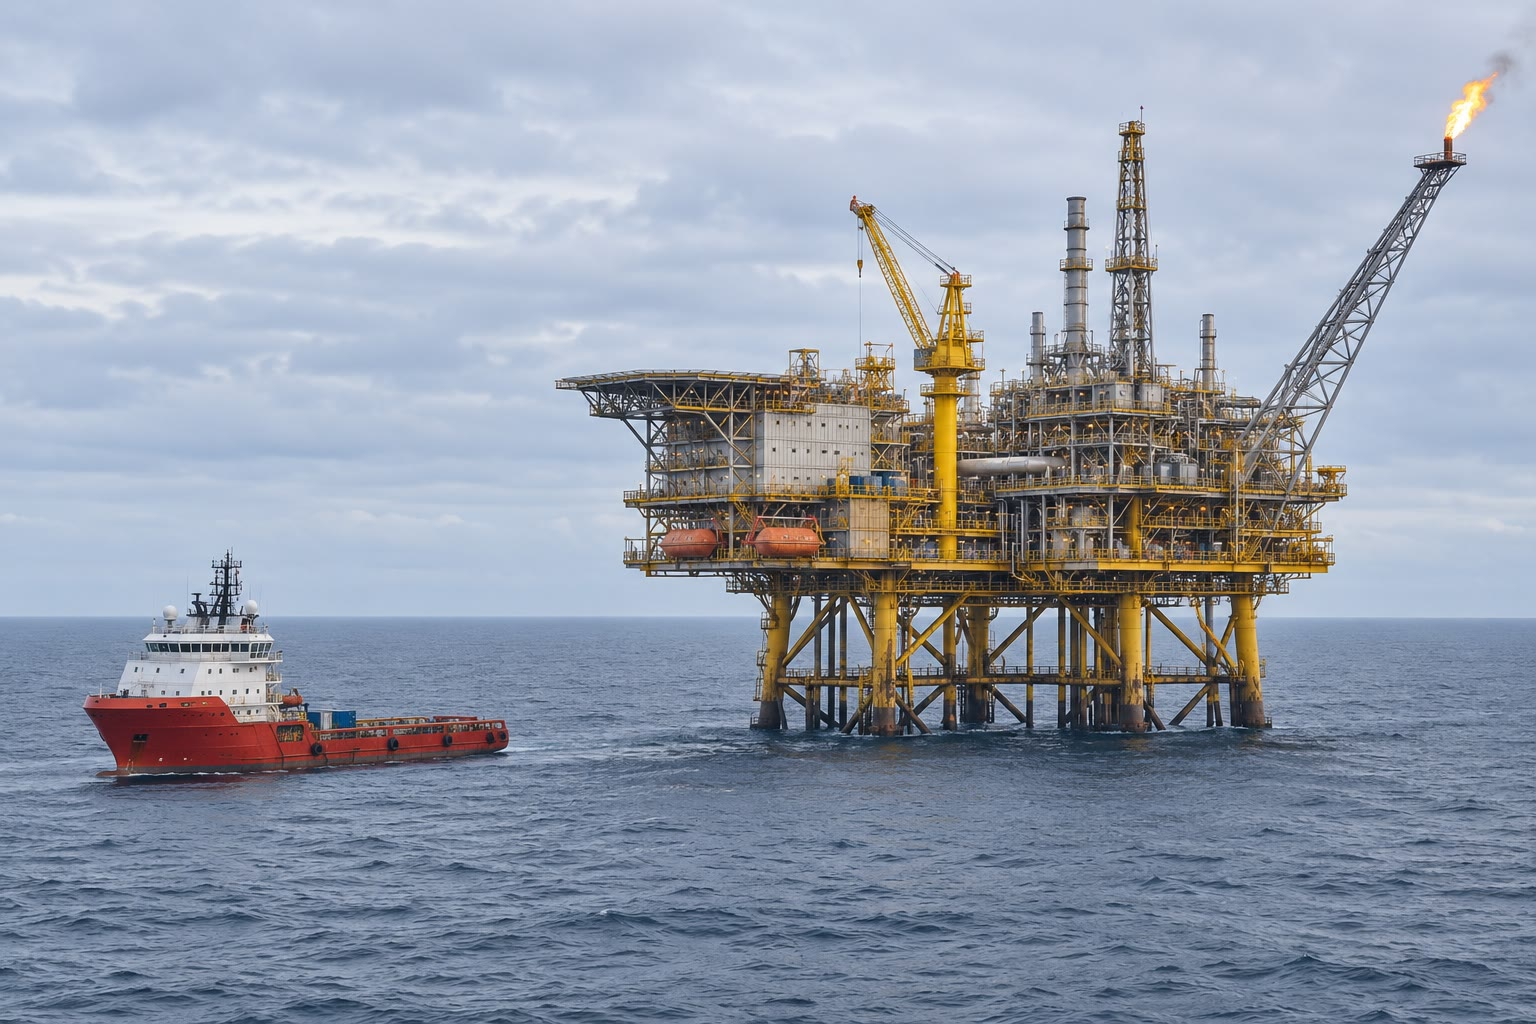
\includegraphics[height=4.4cm]{images/book2/ai/g11-offshore-platform.jpg}

{\small 左：来自宾夕法尼亚一座旧煤矿的富碳页岩化石植物叶片，
时代为石炭纪，页岩板宽约 \qty{10}{cm}。
照片：James St.~John（CC~BY~2.0）。右：海上的石油和天然气生产平台
（AI 插图）。}
\end{omfigure}
% ledger: photo:g11-fossil-plants

\begin{recall}
煤、石油和天然气都是化石燃料：石油和天然气是烃类的混合物，
烃是由碳和氢组成的化合物；燃烧化石燃料会释放能量和二氧化碳
（见化学各册）。植物和藻类借助光合作用，
以二氧化碳和水制造有机物（见生物各册）。
煤、石油和天然气来自埋藏于沉积物中的有机物，并储存于沉积岩中
（第 1 册，九年级）。岩石含有空隙时为多孔的，
水能够流过时为透水的（第 1 册，六年级）。
温度沿\omterm{def:g11:lithosphere-asthenosphere:geotherm}{地温线}随深度升高，
在最初几千米内每千米升高 25 至 \qty{30}{\degreeCelsius}
（见\cref{ch:g11:lithosphere-asthenosphere}）。
\end{recall}
% ledger: usgs:gradient-29, earle:organic-preservation

\section{保存有机物}

绝大多数有机物都不会变成燃料。一片死叶或一种死去的藻类，
会被动物和细菌吃掉，或与空气中的氧气发生反应：几周或几年之内，
其中的碳便以二氧化碳的形式回到大气中。
有机物只有与氧气隔绝时才能保存下来，例如停滞沼泽的底部，
或水中不含氧气的海底与湖底。
有机物被更多沉积物掩埋后，
可以保存数千万乃至数亿年。
% ledger: earle:organic-preservation

煤主要来自堆积于沼泽中的陆生植物。石油和天然气主要来自
海洋中微小的藻类和其他浮游生物：在表层海水生产力很高的地方，
死亡的浮游生物大量降落到海底，速度快到足以使其中一部分
逃脱腐败，并被埋入泥中。
% ledger: earle:coal-formation, earle:oil-window

\begin{definition}[烃源岩；干酪根]\label{def:g11:fossil-fuel-geology:source-rock}
\emph{干酪根}\index{干酪根}是散布于沉积岩中的有机物，
呈细小颗粒，不溶于有机溶剂。
\emph{烃源岩}\index{烃源岩}是富含干酪根的沉积岩，
在被掩埋并受热后，其中形成石油和天然气。
\end{definition}
% ledger: peters08:kerogen, earle:migration-traps

大多数\omterm{def:g11:fossil-fuel-geology:source-rock}{烃源岩}是页岩和泥岩，由富含有机物的泥沉积而成。
在近地表处，其中的\omterm{def:g11:fossil-fuel-geology:source-rock}{干酪根}仍保持固态：生活在无氧环境中的细菌
会把部分有机物转化为甲烷，但其中大部分甲烷会逸散回地表。
生成石油需要热量，而获得热量则需要深度。
% ledger: earle:oil-window, peters08:kerogen

\section{埋藏与成熟}

\begin{definition}[沉积盆地]\label{def:g11:fossil-fuel-geology:basin}
\emph{沉积盆地}\index{沉积盆地}是地壳中
历经数百万年而下沉的区域，沉积物在其中堆积，
厚度常达数千米。
\end{definition}
% ledger: usgs23:rift-salt

在下沉的盆地中，每一层都被不断堆积于其上的地层
埋得越来越深。随着下沉，它沿\omterm{def:g11:lithosphere-asthenosphere:geotherm}{地温线}升温，
即被加热。其中的\omterm{def:g11:fossil-fuel-geology:source-rock}{干酪根}缓慢受热，
大分子断裂为较小的石油和天然气分子。
% ledger: earle:oil-window

\begin{definition}[成熟；生油窗；生气窗]\label{def:g11:fossil-fuel-geology:oil-window}
\emph{成熟}\index{成熟}是\omterm{def:g11:fossil-fuel-geology:source-rock}{烃源岩}中的\omterm{def:g11:fossil-fuel-geology:source-rock}{干酪根}随埋藏和受热
转化为石油和天然气的过程。
\emph{生油窗}\index{生油窗}是温度范围，
约为 60 至 \qty{120}{\degreeCelsius}，在此范围内\omterm{def:g11:fossil-fuel-geology:source-rock}{干酪根}主要生成石油。
超过约 \qty{120}{\degreeCelsius} 后，进入\emph{生气
窗}\index{生气窗}，此时主要生成甲烷。
\end{definition}
% ledger: earle:oil-window, magoon00:tps

由于温度随深度升高，\omterm{def:g11:fossil-fuel-geology:oil-window}{生油窗}同时也是一个深度范围。
当\omterm{def:g11:lithosphere-asthenosphere:geotherm}{地温线}为直线时，该深度范围很容易求出。

\begin{proposition}[生油窗的深度]\label{prop:g11:fossil-fuel-geology:window-depth}
设地表温度为 $T_0$，温度随深度 $z$ 以恒定的\omterm{def:g11:lithosphere-asthenosphere:geotherm}{地温梯度} $G$ 升高：$T = T_0 + G z$。
则\omterm{def:g11:fossil-fuel-geology:oil-window}{生油窗}位于
两深度之间，即
\[
  z_{\text{顶}} = \frac{60 - T_0}{G}
  \qquad\text{和}\qquad
  z_{\text{底}} = \frac{120 - T_0}{G},
\]
式中温度单位为 \unit{\degreeCelsius}。\omterm{def:g11:fossil-fuel-geology:oil-window}{生油窗}的厚度为 $60/G$：
\omterm{def:g11:lithosphere-asthenosphere:geotherm}{地温线}越陡，\omterm{def:g11:fossil-fuel-geology:oil-window}{生油窗}越浅、越薄。
\end{proposition}
% ledger: earle:oil-window

\begin{proof}
顶面位于 $T_0 + G z = 60$ 处，即
$z = (60 - T_0)/G$；底面位于 $T_0 + G z = 120$ 处。二者之差为
$(120 - 60)/G = 60/G$。
\end{proof}

地表温度为 \qty{20}{\degreeCelsius}，\omterm{def:g11:lithosphere-asthenosphere:geotherm}{地温梯度}为
每千米 \qty{30}{\degreeCelsius} 时，\omterm{def:g11:fossil-fuel-geology:oil-window}{生油窗}位于
$40/30 \approx \qty{1.3}{km}$ 与 $100/30 \approx \qty{3.3}{km}$ 之间。美国各地钻孔的
\omterm{def:g11:lithosphere-asthenosphere:geotherm}{地温梯度}平均为
每千米 \qty{29}{\degreeCelsius}，东部为 \num{25}，
西部为 \num{34}。\omterm{def:g11:fossil-fuel-geology:source-rock}{烃源岩}通常需埋藏超过约
\qty{2}{km} 才会生油。若无\omterm{def:g11:fossil-fuel-geology:source-rock}{干酪根}的测定数据，
石油地质学家便将埋藏于较新岩层之下的\omterm{def:g11:fossil-fuel-geology:source-rock}{烃源岩}，
若其上覆较新岩层的厚度超过约 \qty{3}{km}，则视为已\omterm{def:g11:fossil-fuel-geology:oil-window}{成熟}。
% values (oil_window.py): z_top_km 1.3333, z_base_km 3.3333
% ledger: usgs:gradient-29, earle:oil-window, magoon00:tps

\begin{omfigure}
\begin{tikzpicture}
\begin{axis}[omrecord, omage, omdepth, name=burial, width=0.54\linewidth, height=5.6cm,
  xmin=0, xmax=170, ymin=0, ymax=4.5, xlabel={年龄（百万年前）},
  ylabel={深度（\unit{km}）}, unbounded coords=jump, clip=false,
  xtick={0,20,...,160}, ytick={0,1,...,4}]
\fill[omProp!18] (axis cs:170,1.3333) rectangle (axis cs:0,3.3333);
\fill[omThm!12] (axis cs:170,3.3333) rectangle (axis cs:0,4.5);
\node[font=\scriptsize, anchor=west, text=omProp!80!black] at (axis cs:168,1.75) {生油窗};
\node[font=\scriptsize, anchor=west, text=omThm] at (axis cs:168,3.9) {生气窗};
\node[font=\scriptsize, anchor=south west, text=black!60, inner sep=1pt] at (axis cs:168,1.3333) {\qty{60}{\degreeCelsius}};
\node[font=\scriptsize, anchor=south west, text=black!60, inner sep=1pt] at (axis cs:168,3.3333) {\qty{120}{\degreeCelsius}};
% computed in figdata/grade-11/oil_window.py (invented basin)
\addplot[black!45, line width=0.6pt] table[x=age, y=z150] {figdata/out/grade-11-oil_window-history.dat};
\addplot[black!45, line width=0.6pt] table[x=age, y=z120] {figdata/out/grade-11-oil_window-history.dat};
\addplot[black!45, line width=0.6pt] table[x=age, y=z95] {figdata/out/grade-11-oil_window-history.dat};
\addplot[black!45, line width=0.6pt] table[x=age, y=z66] {figdata/out/grade-11-oil_window-history.dat};
\addplot[black, line width=1.4pt] table[x=age, y=z165] {figdata/out/grade-11-oil_window-history.dat};
\draw[omDef, dashed, line width=0.8pt] (axis cs:80,0) -- (axis cs:80,4.5);
\node[font=\scriptsize, anchor=west, text=omDef, inner sep=1pt] at (axis cs:78,4.2) {背斜形成};
\fill[omThm] (axis cs:116.97,1.3333) circle (2pt);
\fill[omThm] (axis cs:51.24,3.3333) circle (2pt);
\node[font=\scriptsize, anchor=north east, inner sep=1pt] at (axis cs:100,2.3) {烃源岩};
\end{axis}
\begin{axis}[omrecord, omdepth, at={(burial.east)}, anchor=west, xshift=1.7cm, width=0.34\linewidth, height=5.6cm,
  xmin=15, xmax=50, ymin=0, ymax=7, xlabel={地温梯度（\unit{\degreeCelsius/km}）},
  ylabel={深度（\unit{km}）}]
% computed in figdata/grade-11/oil_window.py (proposition, surface at 20 degC)
\addplot[name path=top, omProp, line width=1pt] table[x=G, y=z_top] {figdata/out/grade-11-oil_window-windows.dat};
\addplot[name path=base, omThm, line width=1pt] table[x=G, y=z_base] {figdata/out/grade-11-oil_window-windows.dat};
\addplot[omProp!18] fill between[of=top and base];
\node[font=\scriptsize] at (axis cs:40,1.75) {生油窗};
\node[font=\scriptsize, anchor=south, text=omProp!80!black] at (axis cs:42,0.95) {顶};
\node[font=\scriptsize, anchor=north west, text=omThm] at (axis cs:24,4.6) {底};
\end{axis}
\end{tikzpicture}

{\small 左：虚构的梅罗盆地的埋藏史（计算模型，忽略压实作用）。
每条线追踪一层岩层随时间的变化，
自其在地表沉积之日起算；粗线为\omterm{def:g11:fossil-fuel-geology:source-rock}{烃源岩}，
沉积于 1.65 亿年前。地表温度为
\qty{20}{\degreeCelsius}、\omterm{def:g11:lithosphere-asthenosphere:geotherm}{地温梯度}为
每千米 \qty{30}{\degreeCelsius} 时，\omterm{def:g11:fossil-fuel-geology:oil-window}{生油窗}为 \num{1.3} 与
\qty{3.3}{km} 之间的区间。圆点标出\omterm{def:g11:fossil-fuel-geology:source-rock}{烃源岩}进入\omterm{def:g11:fossil-fuel-geology:oil-window}{生油窗}的时间与
离开\omterm{def:g11:fossil-fuel-geology:oil-window}{生油窗}的时间，后者对应\omterm{def:g11:fossil-fuel-geology:oil-window}{生气窗}。右：\omterm{def:g11:fossil-fuel-geology:oil-window}{生油窗}顶部与底部的深度
随\omterm{def:g11:lithosphere-asthenosphere:geotherm}{地温梯度}的变化（地表温度为
\qty{20}{\degreeCelsius}）。}
\end{omfigure}
% values (oil_window.py): enter_oil_Ma 116.97, leave_oil_Ma 51.24, T_max 140 (20 Ma), T_today 125

这样的图称为\emph{埋藏史图}：横轴为年龄，
自左向右指向今天，纵轴为深度，向下递增。它将
逐层定年的岩层柱转化为一段历史。

\begin{method}[读埋藏史图]\label{met:g11:fossil-fuel-geology:burial}
\begin{enumerate}
  \item 找到\omterm{def:g11:fossil-fuel-geology:source-rock}{烃源岩}的线：它从地表开始，
        起点为该岩层沉积之日。
  \item 依据\omterm{def:g11:lithosphere-asthenosphere:geotherm}{地温线}，以深度画出\omterm{def:g11:fossil-fuel-geology:oil-window}{生油窗}的顶部与底部
        （见\cref{prop:g11:fossil-fuel-geology:window-depth}）。
  \item 读出\omterm{def:g11:fossil-fuel-geology:source-rock}{烃源岩}的线穿过窗顶的年龄：
        \omterm{def:g11:fossil-fuel-geology:source-rock}{烃源岩}开始生油。读出其穿过窗底的年龄：
        此后便生气。
  \item 将这些年龄与\omterm{def:g11:fossil-fuel-geology:trap}{圈闭}的年龄相比较：只有在\omterm{def:g11:fossil-fuel-geology:trap}{圈闭}形成之后生成的油气，
        才能被其保存。
\end{enumerate}
\end{method}
% ledger: magoon00:tps

在梅罗盆地中，\omterm{def:g11:fossil-fuel-geology:source-rock}{烃源岩}约于 1.17 亿年前进入\omterm{def:g11:fossil-fuel-geology:oil-window}{生油窗}，
约于 5100 万年前离开\omterm{def:g11:fossil-fuel-geology:oil-window}{生油窗}；其最大埋深
\qty{4.0}{km}、温度 \qty{140}{\degreeCelsius}，出现于 2000 万年前，
之后才因隆升与侵蚀而重新抬升。今天它仍处于
\omterm{def:g11:fossil-fuel-geology:oil-window}{生气窗}中。周末问题将计算这些年龄。
% values (oil_window.py): enter_oil_Ma 116.97, leave_oil_Ma 51.24, z_max_km 4, T_max 140, T_today 125

\section{从烃源岩到圈闭}

油和气的密度小于水，而埋藏岩石的孔隙中
充满了水。油气一旦生成，便被挤出\omterm{def:g11:fossil-fuel-geology:source-rock}{烃源岩}，
穿过任何允许其通过的岩石向上\omterm{def:g11:fossil-fuel-geology:migration}{运移}。
% ledger: earle:migration-traps

\begin{definition}[运移]\label{def:g11:fossil-fuel-geology:migration}
\emph{运移}\index{运移（油气）}是油气
从其生成的\omterm{def:g11:fossil-fuel-geology:source-rock}{烃源岩}中缓慢向上穿过透水岩层的运动，
其动力来自油气密度小于周围水的密度。
\end{definition}
% ledger: earle:migration-traps

\begin{definition}[储集岩；盖层]\label{def:g11:fossil-fuel-geology:reservoir}
\emph{储集岩}\index{储集岩}是一种多孔且透水的岩石，
油气聚集其中：其孔隙储存油气，孔隙间的连通
使油气能够流向水井。\emph{盖层}\index{盖层（盖岩）}是位于储集岩之上的
不透水岩层，
油气无法穿过。
\end{definition}
% ledger: earle:migration-traps, magoon00:tps

砂岩和部分石灰岩是良好的\omterm{def:g11:fossil-fuel-geology:reservoir}{储集岩}；泥岩、页岩和
盐岩是良好的\omterm{def:g11:fossil-fuel-geology:reservoir}{盖层}。若无任何阻挡，油气会上升至
地表，在那里渗出并被氧化：其中的碳回到
大气中。油气只有在\omterm{def:g11:fossil-fuel-geology:reservoir}{盖层}形状使其无法
逸出的地方才会聚集。
% ledger: earle:migration-traps, magoon00:tps

\begin{definition}[圈闭]\label{def:g11:fossil-fuel-geology:trap}
\emph{圈闭}\index{圈闭（油气）}是由\omterm{def:g11:fossil-fuel-geology:reservoir}{储集岩}
和\omterm{def:g11:fossil-fuel-geology:reservoir}{盖层}构成的一种组合，能将油气保留在原处，在各个方向上封闭向上的通道。
\end{definition}
% ledger: earle:migration-traps

\begin{omfigure}
\begin{tikzpicture}[font=\footnotesize, scale=0.95,
    declare function={hz(\x,\c)=\c+0.1*\x+0.7*exp(-((\x-10)^2)/2.5);}]
  \colorlet{omOil}{green!45!black}\colorlet{omGas}{red!65}
  \fill[omLithShale!70!white] (0,0) rectangle (14,-6.3);
  % overburden: limestone above a sandstone
  \fill[omLithCongl!70!white] (0,0) -- (14,0) -- plot[domain=14:0, samples=80] (\x,{-2.4+0.06*\x+0.3*exp(-((\x-10)^2)/2.5)}) -- cycle;
  \fill[omLithSand!60!white] plot[domain=0:14, samples=80] (\x,{-2.4+0.06*\x+0.3*exp(-((\x-10)^2)/2.5)}) -- plot[domain=14:0, samples=80] (\x,{hz(\x,-3.7)}) -- cycle;
  % seal (mudstone)
  \fill[omLithShale] plot[domain=0:14, samples=80] (\x,{hz(\x,-3.7)}) -- plot[domain=14:0, samples=80] (\x,{hz(\x,-4.4)}) -- cycle;
  % reservoir sandstone
  \fill[omLithSand] plot[domain=0:14, samples=80] (\x,{hz(\x,-4.4)}) -- plot[domain=14:0, samples=80] (\x,{hz(\x,-5.0)}) -- cycle;
  % oil and gas in the crest of the anticline, above the spill depth
  \begin{scope}
    \clip plot[domain=0:14, samples=80] (\x,{hz(\x,-4.4)}) -- plot[domain=14:0, samples=80] (\x,{hz(\x,-5.0)}) -- cycle;
    \fill[omOil] (8,-2.97) rectangle (13,-2.6);
    \fill[omGas] (8,-2.81) rectangle (13,-2.6);
  \end{scope}
  % source rock (black shale)
  \fill[black!70] plot[domain=0:14, samples=80] (\x,{hz(\x,-5.0)}) -- plot[domain=14:0, samples=80] (\x,{hz(\x,-5.6)}) -- cycle;
  \foreach \c in {-3.7,-4.4,-5.0,-5.6}
    \draw[black!55, line width=0.4pt] plot[domain=0:14, samples=80] (\x,{hz(\x,\c)});
  \draw[black!55, line width=0.4pt] plot[domain=0:14, samples=80] (\x,{-2.4+0.06*\x+0.3*exp(-((\x-10)^2)/2.5)});
  \draw[black!70] (0,0) -- (14,0);
  % 60 degC isotherm
  \draw[omThm, dashed, line width=0.8pt] (0,-4.3) -- (14,-4.3);
  \node[anchor=north east, text=omThm, fill=omLithShale!70!white, inner sep=1pt] at (13.95,-4.35) {\qty{60}{\degreeCelsius}};
  % migration
  \foreach \s in {0,1}
    \draw[->, omDef, line width=1.1pt] (2.7+1.2*\s,{-5.1+0.12*\s}) -- (3.2+1.2*\s,{-4.55+0.12*\s});
  \draw[->, omDef, line width=1.1pt] (4.6,-4.3) .. controls (6.5,-4.1) and (8.3,-3.7) .. (9.45,-3.0);
  % labels
  \node[anchor=west, text=white] at (0.15,-5.25) {烃源岩};
  \node[anchor=west] at (5.2,-5.75) {温度高于 \qty{60}{\degreeCelsius} 处成熟};
  \node[anchor=west] at (0.15,-4.75) {储集岩};
  \node[anchor=west] at (0.15,-3.97) {盖层};
  \node[anchor=west] at (0.15,-0.4) {上覆岩层};
  \node[anchor=north, text=omDef, fill=omLithShale, inner sep=1pt] at (6.2,-3.62) {迁移};
  \draw[black!60] (10.0,-2.72) -- (11.4,-1.95);
  \node[anchor=south west, fill=omLithSand!60!white, inner sep=1pt] at (11.4,-1.95) {气};
  \draw[black!60] (10.6,-2.88) -- (12.3,-2.55);
  \node[anchor=west, fill=omLithShale, inner sep=1pt] at (12.3,-2.55) {油};
  \draw[black!60] (12.0,-3.45) -- (12.8,-3.15);
  \node[anchor=south, fill=omLithShale, inner sep=1pt] at (12.85,-3.15) {水};
  \node[anchor=north] at (10,-1.0) {圈闭：背斜的拱顶};
\end{tikzpicture}

{\small \omterm{def:g11:fossil-fuel-geology:petroleum-system}{含油气系统}示意图（非按比例绘制）。左侧较深处的\omterm{def:g11:fossil-fuel-geology:source-rock}{烃源岩}
位于 \qty{60}{\degreeCelsius} 等温线之下，生成石油；
石油和天然气从其中迁入上方的砂岩，并沿其缓慢向上渗透，
位于泥岩\omterm{def:g11:fossil-fuel-geology:reservoir}{盖层}之下，直至背斜的拱顶。在那里，流体
按密度分层聚集：气在顶部，油在中部，水在下部。顶部的\omterm{def:g11:fossil-fuel-geology:petroleum-system}{上覆岩层}
将\omterm{def:g11:fossil-fuel-geology:source-rock}{烃源岩}埋藏至足够深度，使其\omterm{def:g11:fossil-fuel-geology:oil-window}{成熟}。}
\end{omfigure}
% ledger: earle:migration-traps, magoon00:tps, earle:oil-window

在\omterm{def:g11:fossil-fuel-geology:trap}{圈闭}中，流体按密度自行分层：气在顶部，油在中部，
水在底部。最简单的\omterm{def:g11:fossil-fuel-geology:trap}{圈闭}是背斜，即岩层中的拱起，
（褶皱是\cref{ch:g12:mountain-building}的内容）。断层、
盐丘以及岩石自身的变化也能形成\omterm{def:g11:fossil-fuel-geology:trap}{圈闭}。
% ledger: earle:migration-traps

\begin{omfigure}
\begin{tikzpicture}[font=\footnotesize, scale=0.78]
  \colorlet{omOil}{green!45!black}\colorlet{omGas}{red!65}
  % (a) anticline
  \begin{scope}
    \fill[omLithShale] (0,0) rectangle (4,3);
    \fill[omLithSand] plot[domain=0:4, samples=50] (\x,{1.0+1.0*exp(-((\x-2)^2)/1.2)}) -- plot[domain=4:0, samples=50] (\x,{1.5+1.0*exp(-((\x-2)^2)/1.2)}) -- cycle;
    \begin{scope}
      \clip plot[domain=0:4, samples=50] (\x,{1.0+1.0*exp(-((\x-2)^2)/1.2)}) -- plot[domain=4:0, samples=50] (\x,{1.5+1.0*exp(-((\x-2)^2)/1.2)}) -- cycle;
      \fill[omOil] (0,1.75) rectangle (4,3); \fill[omGas] (0,2.25) rectangle (4,3);
    \end{scope}
    \draw[black!50] (0,0) rectangle (4,3);
    \node[anchor=north, text height=1.6ex, text depth=0.3ex] at (2,-0.05) {(a) 背斜};
  \end{scope}
  % (b) fault
  \begin{scope}[xshift=4.6cm]
    \fill[omLithShale] (0,0) rectangle (4,3);
    \begin{scope}
      \clip (0,0) -- (2.9,0) -- (2.3,3) -- (0,3) -- cycle;
      \fill[omLithSand] (0,0.6) -- (4,1.8) -- (4,2.3) -- (0,1.1) -- cycle;
      \clip (0,0.6) -- (4,1.8) -- (4,2.3) -- (0,1.1) -- cycle;
      \fill[omOil] (0,1.45) rectangle (4,3); \fill[omGas] (0,1.75) rectangle (4,3);
    \end{scope}
    \begin{scope}
      \clip (2.9,0) -- (4,0) -- (4,3) -- (2.3,3) -- cycle;
      \fill[omLithSand] (0,-0.6) -- (4,0.6) -- (4,1.1) -- (0,-0.1) -- cycle;
    \end{scope}
    \draw[black, line width=1pt] (2.9,0) -- (2.3,3);
    \draw[black!50] (0,0) rectangle (4,3);
    \node[anchor=north, text height=1.6ex, text depth=0.3ex] at (2,-0.05) {(b) 断层};
  \end{scope}
  % (c) salt dome
  \begin{scope}[xshift=9.2cm]
    \fill[omLithShale] (0,0) rectangle (4,3);
    \fill[omLithSand] (0,0.9) -- (1.0,1.2) -- (1.4,1.9) -- (1.4,2.4) -- (1.0,1.7) -- (0,1.4) -- cycle;
    \fill[omLithSand] (4,0.9) -- (3.0,1.2) -- (2.6,1.9) -- (2.6,2.4) -- (3.0,1.7) -- (4,1.4) -- cycle;
    \begin{scope}
      \clip (0,0.9) -- (1.0,1.2) -- (1.4,1.9) -- (1.4,2.4) -- (1.0,1.7) -- (0,1.4) -- cycle;
      \fill[omOil] (0,1.65) rectangle (1.4,3); \fill[omGas] (0,2.05) rectangle (1.4,3);
    \end{scope}
    \begin{scope}
      \clip (4,0.9) -- (3.0,1.2) -- (2.6,1.9) -- (2.6,2.4) -- (3.0,1.7) -- (4,1.4) -- cycle;
      \fill[omOil] (2.6,1.65) rectangle (4,3); \fill[omGas] (2.6,2.05) rectangle (4,3);
    \end{scope}
    \fill[omLithEvap, draw=black!60] (1.4,0) -- (1.4,2.4) .. controls (1.4,2.85) and (2.6,2.85) .. (2.6,2.4) -- (2.6,0) -- cycle;
    \node at (2,1.0) {盐};
    \draw[black!50] (0,0) rectangle (4,3);
    \node[anchor=north, text height=1.6ex, text depth=0.3ex] at (2,-0.05) {(c) 盐丘};
  \end{scope}
  % (d) stratigraphic
  \begin{scope}[xshift=13.8cm]
    \fill[omLithShale] (0,0) rectangle (4,3);
    \fill[omLithSand] (0,0.6) -- (3.5,1.95) -- (0,1.3) -- cycle;
    \begin{scope}
      \clip (0,0.6) -- (3.5,1.95) -- (0,1.3) -- cycle;
      \fill[omOil] (0,1.45) rectangle (4,3); \fill[omGas] (0,1.7) rectangle (4,3);
    \end{scope}
    \draw[black!50] (0,0) rectangle (4,3);
    \node[anchor=north, text height=1.6ex, text depth=0.3ex] at (2,-0.05) {(d) 尖灭};
  \end{scope}
\end{tikzpicture}

{\small 四种\omterm{def:g11:fossil-fuel-geology:trap}{圈闭}（示意图，不按比例）：储层砂岩为黄色，
\omterm{def:g11:fossil-fuel-geology:reservoir}{盖层}泥岩为灰绿色，石油为绿色，天然气为红色。（a）
背斜的拱部。（b）倾斜的储层被断层切割，
另一侧与泥岩相接。（c）岩层向上弯曲，贴靠在隆起的盐丘上。
（d）砂岩在泥岩中向上坡方向逐渐尖灭，
是由岩石本身的变化形成的\omterm{def:g11:fossil-fuel-geology:trap}{圈闭}。}
\end{omfigure}
% ledger: earle:migration-traps

\begin{example}[背斜中的圈闭]\label{ex:g11:fossil-fuel-geology:anticline}
地震勘测绘出了被泥岩\omterm{def:g11:fossil-fuel-geology:reservoir}{盖层}封闭的砂岩顶面。它呈拱形，
拱顶位于地表以下 \qty{1800}{m}。拱顶周围，
仍能完全闭合的最深等高线位于
\qty{2050}{m} 处；在其下方，砂岩向侧面开放。拱顶处的一口井
在 \qty{1880}{m} 深度以上见到天然气。该\omterm{def:g11:fossil-fuel-geology:trap}{圈闭}能容纳多高的油气柱，
其中石油层有多厚？

\emph{解。}油气自拱顶向下充满拱形构造；任何
沉到最后一条闭合等高线以下的油气，会从侧面溢出，在
\emph{溢出点}处溢出并继续迁移。油气柱的最大高度为
$2050 - 1800 = \qty{250}{m}$。若\omterm{def:g11:fossil-fuel-geology:trap}{圈闭}被充满，天然气充填顶部
$1880 - 1800 = \qty{80}{m}$ 段，石油充填其下的 $2050 - 1880 = \qty{170}{m}$ 段，
下方为水。
\end{example}
% invented numbers; ledger: earle:migration-traps

下列各部分——\omterm{def:g11:fossil-fuel-geology:source-rock}{烃源岩}、\omterm{def:g11:fossil-fuel-geology:reservoir}{储集岩}、\omterm{def:g11:fossil-fuel-geology:reservoir}{盖层}、埋藏\omterm{def:g11:fossil-fuel-geology:source-rock}{烃源岩}的\omterm{def:g11:fossil-fuel-geology:petroleum-system}{上覆岩层}、
\omterm{def:g11:fossil-fuel-geology:trap}{圈闭}——都是必需的，且必须按
正确的顺序出现。

\begin{definition}[含油气系统]\label{def:g11:fossil-fuel-geology:petroleum-system}
\emph{含油气系统}\index{含油气系统}是指一套\omterm{def:g11:fossil-fuel-geology:oil-window}{成熟}\omterm{def:g11:fossil-fuel-geology:source-rock}{烃源岩}，
连同由其生成的全部油气，以及所需的要素与过程：
\omterm{def:g11:fossil-fuel-geology:source-rock}{烃源岩}、\omterm{def:g11:fossil-fuel-geology:reservoir}{储集岩}、\omterm{def:g11:fossil-fuel-geology:reservoir}{盖层}和
\emph{上覆岩层}\index{上覆岩层}（位于其上、埋藏\omterm{def:g11:fossil-fuel-geology:source-rock}{烃源岩}的岩层），
\omterm{def:g11:fossil-fuel-geology:trap}{圈闭}的形成，
以及油气的生成、\omterm{def:g11:fossil-fuel-geology:migration}{运移}与聚集。
\end{definition}
% ledger: magoon00:tps

次序最为关键。形成于油气已经离开之后的\omterm{def:g11:fossil-fuel-geology:trap}{圈闭}，
什么也捕获不到：埋藏史图可确定石油的生成时间，
褶皱与断层的历史可确定\omterm{def:g11:fossil-fuel-geology:trap}{圈闭}的形成时间，\omterm{def:g11:fossil-fuel-geology:petroleum-system}{含油气系统}只有在
\omterm{def:g11:fossil-fuel-geology:trap}{圈闭}先于油气形成时才能成立。石油地质学家还把最能同时体现
生成、\omterm{def:g11:fossil-fuel-geology:migration}{运移}与聚集的时间称为\emph{关键
时刻}。
% ledger: magoon00:tps

\section{油气聚集于何处}

\omterm{def:g11:fossil-fuel-geology:petroleum-system}{含油气系统}在何处形成？它需要一个长期沉降的盆地，
水体缺氧以保存有机质，并需要\omterm{def:g11:fossil-fuel-geology:reservoir}{盖层}。裂谷
及其发展而成的大陆边缘同时具备这三个条件。
% ledger: usgs23:rift-salt

当一个大陆开始裂解时，正如今日的非洲沿东
非裂谷（第 1 册，七年级）所示，地壳拉伸并破裂为块体，
沿\omterm{def:g11:ocean-ridges:normal-fault}{正断层}（见\cref{ch:g11:ocean-ridges}）发育。部分块体下降，
另一些倾斜，块体之间的凹槽被沉积物充填，厚度常达数千米，
并有湖泊相伴，湖中富含有机质的泥质沉积可
成为\omterm{def:g11:fossil-fuel-geology:source-rock}{烃源岩}。当
拉伸停止后，减薄的地壳冷却并持续缓慢下沉，因而
盆地继续充填。若海水随后侵入仅部分
与大洋相连的盆地并发生蒸发，便会留下厚层的
盐层。裂谷一旦张开形成大洋，其边缘便成为被动
大陆边缘，即位于板块内部、远离任何板块边界的大陆边缘，它们
持续下沉，并接受来自陆地的沉积物。
% ledger: usgs23:rift-salt, usgs:pangaea-breakup

\begin{omfigure}
\begin{tikzpicture}[font=\footnotesize, x=1cm, y=0.8cm]
  \fill[omLithShale] (0,0.25) -- (1.5,0) -- (7,-0.4) -- (10,-2.2) -- (14,-2.6) -- (14,-8.0) -- (0,-8.0) -- cycle;
  % sea and land
  \fill[omSea] (1.5,0) -- (14,0) -- (14,-2.6) -- (10,-2.2) -- (7,-0.4) -- cycle;
  \draw[omRiver!60, line width=0.6pt] (1.5,0) -- (14,0);
  % marine sediments above the salt
  \fill[omLithShale] (0,0.25) -- (1.5,0) -- (7,-0.4) -- (10,-2.2) -- (14,-2.6) -- (14,-4.95) -- (11.2,-4.5) -- (11.2,-3.74) -- (0,-2.4) -- cycle;
  \fill[omLithSand] (0,-0.9) -- (6,-1.45) -- (10,-2.75) -- (14,-3.3) -- (14,-3.6) -- (10,-3.05) -- (6,-1.75) -- (0,-1.2) -- cycle;
  % salt layer and a salt dome
  \fill[omLithEvap, draw=black!50] (1.2,-2.25) -- (11.2,-3.74) -- (11.2,-4.14) -- (1.2,-2.65) -- cycle;
  \fill[omLithEvap, draw=black!50] (7.0,-3.0) .. controls (7.3,-2.6) and (7.25,-1.9) .. (7.2,-1.6)
     .. controls (7.4,-1.2) and (8.2,-1.2) .. (8.4,-1.6)
     .. controls (8.35,-2.1) and (8.3,-2.7) .. (8.7,-3.25) -- cycle;
  % continental crust with tilted blocks
  \fill[omLithGranite] (0,-2.75) -- (2.5,-3.0) -- (4.85,-4.6) -- (5.0,-3.4) -- (7.35,-5.0) -- (7.5,-3.75) -- (9.85,-5.3) -- (10.0,-4.1) -- (11.2,-5.0) -- (11.2,-6.0) -- (0,-7.6) -- cycle;
  % rift fill: lake shales (source rocks) in the half-grabens
  \fill[black!65] (2.5,-3.0) -- (4.85,-4.6) -- (5.0,-3.4) -- (4.0,-3.25) -- cycle;
  \fill[black!65] (5.0,-3.4) -- (7.35,-5.0) -- (7.5,-3.75) -- (6.5,-3.6) -- cycle;
  \fill[black!65] (7.5,-3.75) -- (9.85,-5.3) -- (10.0,-4.1) -- (9.0,-3.95) -- cycle;
  \fill[black!65] (2.5,-3.0) -- (4.0,-3.25) -- (5.0,-3.4) -- (6.5,-3.6) -- (7.5,-3.75) -- (9.0,-3.95) -- (10.0,-4.1) -- (11.2,-4.3) -- (11.2,-4.14) -- (1.2,-2.65) -- (1.2,-2.87) -- cycle;
  \draw[black!70, line width=0.8pt] (4.85,-4.6) -- (5.0,-3.4) (7.35,-5.0) -- (7.5,-3.75) (9.85,-5.3) -- (10.0,-4.1);
  % oceanic crust and mantle
  \fill[omLithBasalt] (11.2,-4.5) -- (14,-4.95) -- (14,-6.0) -- (11.2,-6.0) -- cycle;
  \fill[omLithPeridotite] (0,-7.6) -- (11.2,-6.0) -- (14,-6.0) -- (14,-8.0) -- (0,-8.0) -- cycle;
  % oil beside the salt dome
  \fill[green!45!black] (6.85,-1.5) -- (7.22,-1.65) -- (7.22,-1.95) -- (6.85,-1.75) -- cycle;
  \draw[black!60] (0,-8.0) rectangle (14,1.0);
  % labels
  \node[anchor=west] at (11.5,-1.2) {海};
  \node[anchor=south west] at (0.1,0.3) {陆地};
  \node[anchor=west, fill=omLithShale, inner sep=1pt] at (2.2,-0.45) {海相沉积};
  \node[anchor=west, fill=omLithEvap, inner sep=1pt] at (9.0,-1.25) {盐丘};
  \draw[black!60] (8.4,-1.4) -- (9.0,-1.25);
  \node[anchor=east, fill=omLithShale, inner sep=1pt] at (6.6,-2.1) {石油};
  \draw[black!60] (6.6,-2.1) -- (6.95,-1.75);
  \node[anchor=west, fill=omLithShale, inner sep=1pt] at (11.4,-3.35) {盐层（盖层）};
  \draw[black!60] (10.8,-3.7) -- (11.4,-3.35);
  \node[anchor=west, align=left] at (0.3,-4.7) {湖相页岩 \\（烃源岩）};
  \draw[black!60] (2.75,-4.45) -- (4.4,-3.8);
  \node[anchor=north, align=center] at (4.0,-5.6) {拉伸的陆壳：\\倾斜块体与正断层};
  \node[anchor=north, align=center] at (12.6,-5.05) {洋壳};
  \node[anchor=north] at (6,-7.35) {地幔};
\end{tikzpicture}

{\small 建于古老裂谷之上的被动大陆边缘（示意图，未按比例，
深度经夸大）。裂谷中，由\omterm{def:g11:ocean-ridges:normal-fault}{正断层}围限的大陆地壳倾斜块体
中保存着湖相页岩，即\omterm{def:g11:fossil-fuel-geology:source-rock}{烃源岩}。一层盐岩在年轻海洋蒸发时沉积，
封存了它们；其上，海相沉积物随边缘下沉而不断堆积。
盐的密度小于周围沉积物，因而上升，
形成盐丘，使地层弯曲而形成\omterm{def:g11:fossil-fuel-geology:trap}{圈闭}。}
\end{omfigure}
% ledger: usgs23:rift-salt, earle:migration-traps

南大西洋两岸的大陆边缘即以此方式形成。非洲与南美洲
大约在晚三叠世或早侏罗世开始分离。中非西部近海，
裂谷槽中充填了数千米沉积物，其中包括
湖相页岩，厚达 \qty{600}{m}，有机碳质量分数高达
\qty{20}{\percent}。早白垩世时，海水
开始反复侵入并蒸发，留下超过 1 千米厚的盐层；
盐层仍保留原位的地方，它封存了下方岩层中的石油
和天然气。在墨西哥湾，密度小于周围沉积物的盐
向上升起形成盐丘，与之相接的地层弯曲，
形成\omterm{def:g11:fossil-fuel-geology:trap}{圈闭}。
% ledger: usgs23:rift-salt, earle:migration-traps

\section{煤}

煤形成于陆地上，多见于河流与三角洲旁的沼泽中，形成环境为潮湿
气候，从热带到温带皆有，植物生长迅速，其遗体
落入缺氧的静水中。经历数百至数千年，它们逐渐堆积
成泥炭。河流改道或海平面上升时，沙与泥将泥炭掩埋；
埋得更深后，泥炭受到挤压和加热。
% ledger: earle:coal-formation

\begin{definition}[煤；煤化作用；煤阶]\label{def:g11:fossil-fuel-geology:coal}
\emph{煤}\index{煤}是一种主要由陆生植物遗体构成的沉积岩，
富含碳。\emph{煤化作用}\index{煤化作用}是泥炭转变为煤、煤转变为
更富碳煤的过程，依靠埋藏和加热实现。
\emph{煤阶}\index{煤阶}指煤的煤化程度，
即煤化作用进行的程度：从褐煤经次烟煤、烟煤到无烟煤，
碳含量逐渐升高。
\end{definition}
% ledger: earle:coal-formation, eia:coal-carbon

褐煤形成于几百米至约 \qty{1.5}{km} 的深度，
温度可达约 \qty{50}{\degreeCelsius}；烟煤形成于 1 至
\qty{5}{km} 的深度，温度可达约 \qty{150}{\degreeCelsius}；无烟煤则
形成于超过 \qty{5}{km} 且 \qty{150}{\degreeCelsius} 的条件下。随着\omterm{def:g11:fossil-fuel-geology:coal}{煤阶}升高，
碳在煤中所占比例越来越高：褐煤中约为
25 至 \qty{35}{\percent}，无烟煤中则可达 86 至 \qty{97}{\percent}。
甲烷在形成过程中生成，保留在煤的孔隙中，
这也是煤矿可能含有爆炸性气体的原因。形成一层煤层需要
数百万年。
% ledger: earle:coal-formation, eia:coal-carbon

\begin{omfigure}
\begin{tikzpicture}
\begin{axis}[omrecord, xbar, name=rank, width=0.5\linewidth, height=4.6cm, xmin=0, xmax=100,
  ymin=0.4, ymax=4.6, ytick={1,2,3,4},
  yticklabels={褐煤, 次烟煤, 烟煤, 无烟煤},
  xlabel={碳含量（\unit{\percent}）}, ymajorgrids=false]
% ledger: eia:coal-carbon
\fill[omProp!60!black!35] (axis cs:25,0.7) rectangle (axis cs:35,1.3);
\fill[omProp!70!black!55] (axis cs:35,1.7) rectangle (axis cs:45,2.3);
\fill[black!60] (axis cs:45,2.7) rectangle (axis cs:86,3.3);
\fill[black!85] (axis cs:86,3.7) rectangle (axis cs:97,4.3);
\node[font=\scriptsize, anchor=west] at (axis cs:36,1) {25--35};
\node[font=\scriptsize, anchor=west] at (axis cs:46,2) {35--45};
\node[font=\scriptsize, anchor=east, text=white] at (axis cs:85,3) {45--86};
\node[font=\scriptsize, anchor=east] at (axis cs:85,4) {86--97};
\end{axis}
\node[anchor=west] at ([xshift=0.6cm]rank.east) {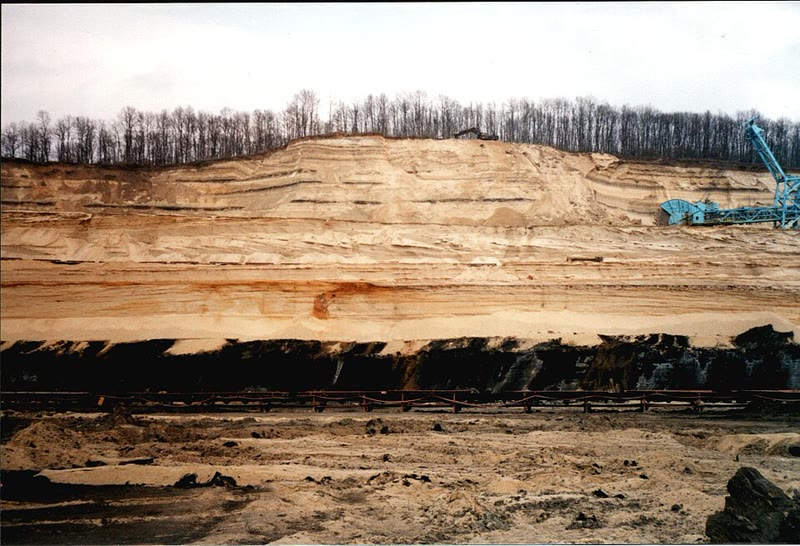
\includegraphics[height=4.0cm]{images/book2/g11-usgs-lignite-bed.jpg}};
\end{tikzpicture}

\medskip
\makebox[0.32\linewidth]{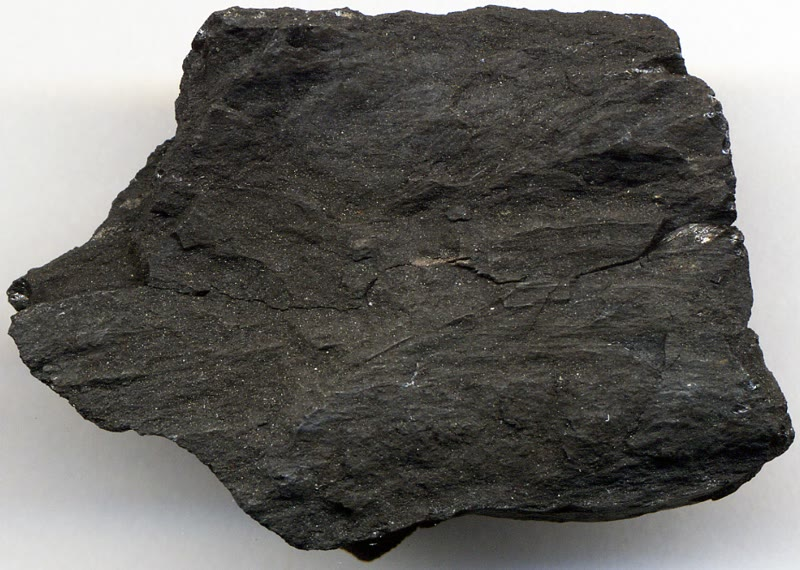
\includegraphics[height=3.2cm]{images/book2/g11-stjohn-lignite.jpg}}\hfill
\makebox[0.32\linewidth]{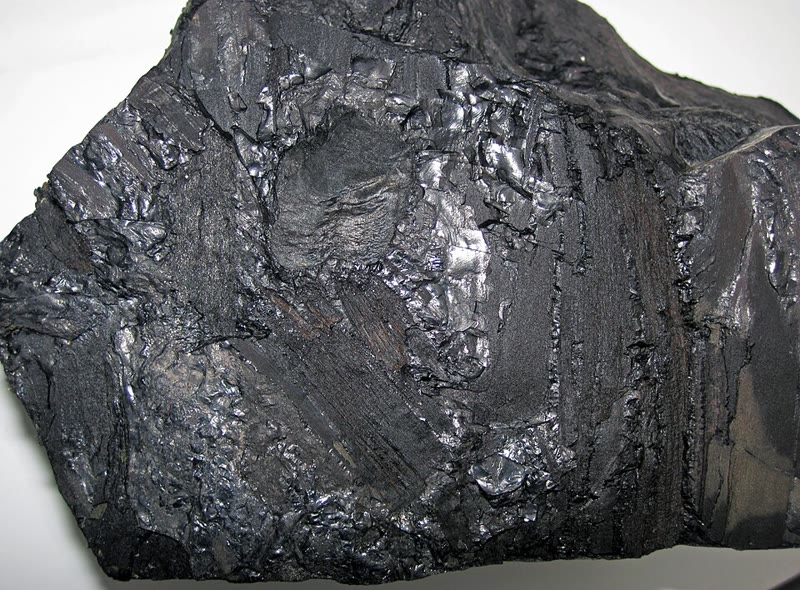
\includegraphics[height=3.2cm]{images/book2/g11-stjohn-bituminous.jpg}}\hfill
\makebox[0.32\linewidth]{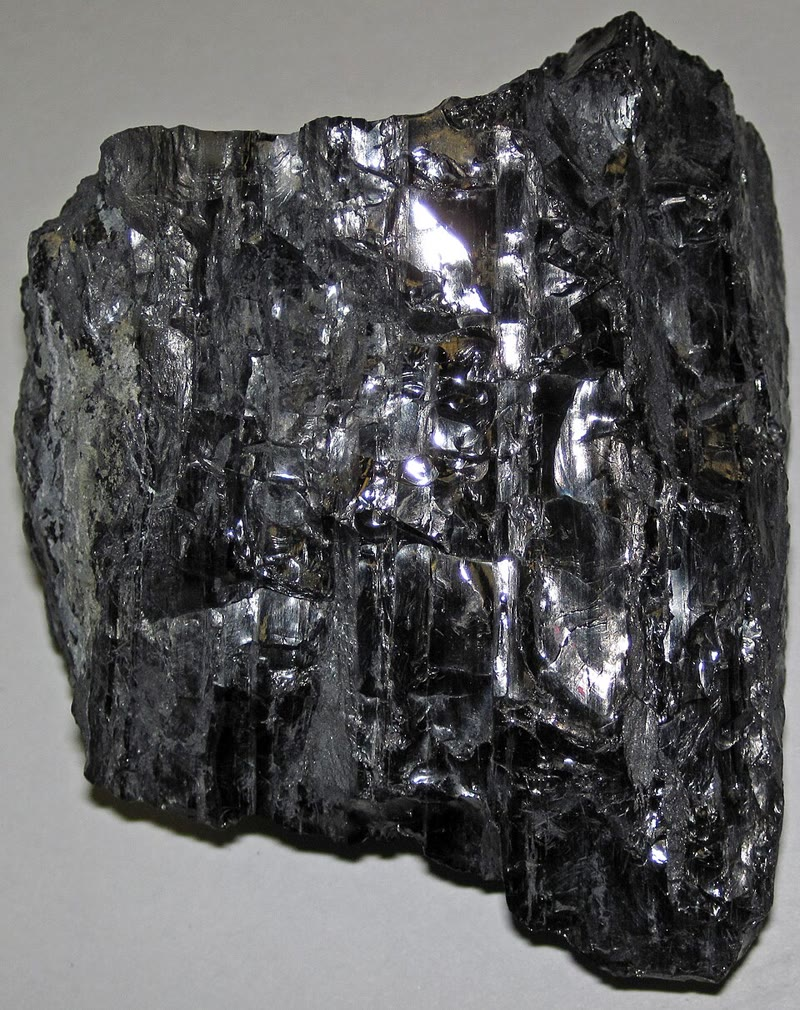
\includegraphics[height=3.2cm]{images/book2/g11-stjohn-anthracite.jpg}}

{\small 左上：各\omterm{def:g11:fossil-fuel-geology:coal}{煤阶}的碳含量。数据来源：美国能源信息署。右上：
褐煤层，即浅色砂层下方的黑色条带，露于罗马尼亚一座矿山中；
照片：美国地质调查局（公有领域）。下排从左至右：
褐煤，约 \qty{4.5}{cm} 宽，棕黑色、暗淡无光；烟煤，带有扁平
的植物碎片；
无烟煤，黑色、呈玻璃\omterm{def:g11:minerals:lustre}{光泽}。照片：James St.~John
（CC~BY~2.0）。}
\end{omfigure}
% ledger: eia:coal-carbon, photo:g11-lignite-bed, photo:g11-coal-ranks

泥炭在转变过程中会损失大部分体积。在美国犹他州中部某煤层中，
将古河道切走的泥炭与旁边缺失的煤层进行比较，
可得厚度之比约为 $11{:}1$：该烟煤每一米，
原先约相当于 11 米泥炭。
% ledger: ryer80:peat-coal

\section{练习}

\begin{exercise}[$\star$]\label{exo:g11:fossil-fuel-geology:1}
将下列由浮游生物形成\omterm{def:g11:fossil-fuel-geology:trap}{圈闭}中石油的步骤按顺序排列：迁移；
在\omterm{def:g11:fossil-fuel-geology:oil-window}{生油窗}内\omterm{def:g11:fossil-fuel-geology:oil-window}{成熟}；被较新的沉积物埋藏；死亡的浮游生物
沉降于缺氧的海底；石油聚集于\omterm{def:g11:fossil-fuel-geology:reservoir}{盖层}之下；有机质在泥中
转变为\omterm{def:g11:fossil-fuel-geology:source-rock}{干酪根}。
\end{exercise}

\begin{exercise}[$\star$]\label{exo:g11:fossil-fuel-geology:2}
判断下列每种岩石最可能属于\omterm{def:g11:fossil-fuel-geology:source-rock}{烃源岩}、\omterm{def:g11:fossil-fuel-geology:reservoir}{储集岩}还是
\omterm{def:g11:fossil-fuel-geology:reservoir}{盖层}：(1) 富含有机质的暗色页岩；(2) 分选良好的
孔隙连通的砂岩；(3) 一层盐；(4) 不含有机质的泥岩；
(5) 充满开放孔洞的石灰岩。
\end{exercise}

\begin{exercise}[$\star$]\label{exo:g11:fossil-fuel-geology:3}
某盆地的地表温度为 \qty{10}{\degreeCelsius}，\omterm{def:g11:lithosphere-asthenosphere:geotherm}{地温梯度}为
\qty{25}{\degreeCelsius/km}。\omterm{def:g11:fossil-fuel-geology:oil-window}{生油窗}位于哪两个深度之间？
其厚度是多少？
\end{exercise}

\begin{exercise}[$\star$]\label{exo:g11:fossil-fuel-geology:4}
(1) 将褐煤、无烟煤、烟煤和泥炭按煤级由低到高排列。
(2) 哪种煤的碳含量最高？(3) 哪种煤形成于
最大深度和最高温度条件下？
\end{exercise}

\begin{exercise}[$\star$]\label{exo:g11:fossil-fuel-geology:5}
(1) 在\omterm{def:g11:fossil-fuel-geology:trap}{圈闭}中，为什么天然气位于石油之上、石油位于水之上？(2) 为什么
\omterm{def:g11:fossil-fuel-geology:reservoir}{储集岩}之上的岩层必须不透水？请举出
两种可作良好\omterm{def:g11:fossil-fuel-geology:reservoir}{盖层}的岩石。
\end{exercise}

\begin{exercise}[$\star\star$]\label{exo:g11:fossil-fuel-geology:6}
两个盆地的地表温度相同，均为 \qty{15}{\degreeCelsius}。
盆地 A 的\omterm{def:g11:lithosphere-asthenosphere:geotherm}{地温梯度}为 \qty{20}{\degreeCelsius/km}，盆地 B 为
\qty{40}{\degreeCelsius/km}。(1) 分别计算两盆地中
\omterm{def:g11:fossil-fuel-geology:oil-window}{生油窗}顶部和底部的深度。(2) \omterm{def:g11:fossil-fuel-geology:source-rock}{烃源岩}在两盆地中均位于 \qty{2}{km} 深处，
各自生成什么？(3) 在哪个盆地中，井须钻得更深
才能找到原地生成的石油？
\end{exercise}

\begin{exercise}[$\star\star$]\label{exo:g11:fossil-fuel-geology:7}
取在犹他州中部测得的泥炭厚度与其所变成煤层厚度的比值 $11{:}1$。
(1) 多厚的泥炭能形成
厚 \qty{3}{m} 的煤层？(2) 假设泥炭以每年 \qty{1}{mm} 的速度堆积，
需要多长时间才能积累形成？(3) 为什么沼泽在这段时间内
必定一直在下沉？
\end{exercise}

\begin{exercise}[$\star\star$]\label{exo:g11:fossil-fuel-geology:8}
利用默罗盆地的埋藏史图（地表温度 \qty{20}{\degreeCelsius}，
\omterm{def:g11:lithosphere-asthenosphere:geotherm}{地温梯度} \qty{30}{\degreeCelsius/km}）。该\omterm{def:g11:fossil-fuel-geology:source-rock}{烃源岩}
在 1.2 亿年前埋深 \qty{1.2}{km}，9500 万年前埋深 \qty{2.3}{km}，
2000 万年前埋深 \qty{4.0}{km}。(1) 计算
其在各时刻的温度。(2) 在各时刻，它处于未\omterm{def:g11:fossil-fuel-geology:oil-window}{成熟}阶段、\omterm{def:g11:fossil-fuel-geology:oil-window}{生油窗}还是
\omterm{def:g11:fossil-fuel-geology:oil-window}{生气窗}？
\end{exercise}

\begin{exercise}[$\star\star$]\label{exo:g11:fossil-fuel-geology:9}
某储集砂岩的顶面形成一个拱形，其脊顶埋深 \qty{2400}{m}；
其最深的闭合等值线位于 \qty{2580}{m}。一口井在脊顶处
钻到 \qty{2450}{m} 处见气，再往下见油。(1) 该\omterm{def:g11:fossil-fuel-geology:trap}{圈闭}能容纳的最大
油柱高度是多少？(2) 若\omterm{def:g11:fossil-fuel-geology:trap}{圈闭}已充满，油层厚度为多少？
(3) \omterm{def:g11:fossil-fuel-geology:trap}{圈闭}充满之后仍不断\omterm{def:g11:fossil-fuel-geology:migration}{运移}来的油和气
去向如何？
\end{exercise}

\begin{exercise}[$\star\star$]\label{exo:g11:fossil-fuel-geology:10}
在无法测定\omterm{def:g11:fossil-fuel-geology:source-rock}{干酪根}时，石油地质学家把\omterm{def:g11:fossil-fuel-geology:petroleum-system}{上覆岩层}厚度超过
\qty{3}{km} 的\omterm{def:g11:fossil-fuel-geology:source-rock}{烃源岩}视为已\omterm{def:g11:fossil-fuel-geology:oil-window}{成熟}。
地表温度为 \qty{20}{\degreeCelsius}。(1) 哪种\omterm{def:g11:lithosphere-asthenosphere:geotherm}{地温梯度}使
\qty{3}{km} 恰位于\omterm{def:g11:fossil-fuel-geology:oil-window}{生油窗}顶部，又恰位于其底部？(2) 利用钻孔中测得的
25 至 \qty{34}{\degreeCelsius/km} 的\omterm{def:g11:lithosphere-asthenosphere:geotherm}{地温梯度}，\qty{3}{km} 深度落在何处？
该规则是否合理？
\end{exercise}

\begin{exercise}[$\star\star$]\label{exo:g11:fossil-fuel-geology:11}
三个煤样的碳含量分别为 \qty{30}{\percent}、\qty{70}{\percent} 和
\qty{92}{\percent}。(1) 给出每个煤样的煤级。(2) 利用课文给出的
深度与温度，哪一个埋藏最深？
(3) 褐煤外观暗淡、呈褐黑色，无烟煤的外观如何？
\end{exercise}

\begin{exercise}[$\star\star\star$]\label{exo:g11:fossil-fuel-geology:12}
在 1.2 亿年前至 9500 万年前之间，\qty{1100}{m} 厚的泥堆积于
默罗盆地。(1) 计算以米每百万年计的埋藏速率。
(2) \omterm{def:g11:lithosphere-asthenosphere:geotherm}{地温梯度}为 \qty{30}{\degreeCelsius/km}，\omterm{def:g11:fossil-fuel-geology:source-rock}{烃源岩}每百万年
升温多少度？(3) 若该速率持续不变，\omterm{def:g11:fossil-fuel-geology:source-rock}{烃源岩}
穿越整个\omterm{def:g11:fossil-fuel-geology:oil-window}{生油窗}需要多长时间？(4) 模型给出约
6600 万年，为何更长？
\end{exercise}

\begin{exercise}[$\star\star\star$]\label{exo:g11:fossil-fuel-geology:13}
在默罗盆地中，\omterm{def:g11:fossil-fuel-geology:source-rock}{烃源岩}约自 1.17 亿年前起处于\omterm{def:g11:fossil-fuel-geology:oil-window}{生油窗}内，
至约 5100 万年前，捕获石油的背斜形成于
8000 万年前。(1) 假设\omterm{def:g11:fossil-fuel-geology:source-rock}{烃源岩}在\omterm{def:g11:fossil-fuel-geology:oil-window}{生油窗}内以稳定速率生成石油，
在\omterm{def:g11:fossil-fuel-geology:oil-window}{生油窗}内期间，其石油中有多大比例形成于
\omterm{def:g11:fossil-fuel-geology:trap}{圈闭}已存在之后？(2) 其余的油去向如何？(3) 若背斜
形成于 4000 万年前，它能容纳多少石油？
\end{exercise}

\begin{exercise}[$\star\star\star$]\label{exo:g11:fossil-fuel-geology:14}
取默罗盆地的埋藏史（见\cref{exo:g11:fossil-fuel-geology:8}：
1.5 亿年前埋深 \qty{0.4}{km}，1.2 亿年前 \qty{1.2}{km}，9500 万年前 \qty{2.3}{km}，
6600 万年前 \qty{3.0}{km}，其间深度稳步增加），本盆地更热：
\omterm{def:g11:lithosphere-asthenosphere:geotherm}{地温梯度} \qty{40}{\degreeCelsius/km}，地表温度为
\qty{20}{\degreeCelsius}。(1) 计算\omterm{def:g11:fossil-fuel-geology:oil-window}{生油窗}顶部和底部的深度。(2) 计算
\omterm{def:g11:fossil-fuel-geology:source-rock}{烃源岩}进入和离开\omterm{def:g11:fossil-fuel-geology:oil-window}{生油窗}的时代。(3) 背斜仍形成于
8000 万年前，它能否容纳石油？
能否容纳天然气？
\end{exercise}

\begin{exercise}[$\star\star\star$]\label{exo:g11:fossil-fuel-geology:15}
一层石炭纪无烟煤目前出露于地表。
石炭纪约于 2.99 亿年前结束。(1) 利用课文给出的深度，
该煤层至少曾埋藏于多深？(2) 地表温度为
\qty{15}{\degreeCelsius}，\omterm{def:g11:lithosphere-asthenosphere:geotherm}{地温梯度}为 \qty{30}{\degreeCelsius/km}，
则该深度处的温度为多少？是否与无烟煤给出的温度一致？(3) 其上方
的岩层经历了什么？假设变化全部发生在石炭纪之后，
给出平均速率的下限，单位为毫米
每年。
\end{exercise}

\section{问题：烃源岩何时生成石油？}

\begin{problem}[{周末问题——为一个虚构盆地的石油定年}]
\label{pb:g11:fossil-fuel-geology:1}
% values (oil_window.py): enter_oil_Ma 116.97, leave_oil_Ma 51.238, T_max 140, T_today 125,
% after_trap_frac 0.43757; ledger ics:base.Jurassic, ics:base.Cretaceous, earle:*, magoon00:tps
一口井钻穿默罗盆地背斜的脊顶，
这是一个虚构盆地，井穿过其下伏各层，由化石测定年代，它们
记录了盆地的充填过程。自最老的一层起：
\begin{center}
\small
\begin{tabular}{|l|l|l|}
\hline
\textbf{时间段（百万年前）} & \textbf{厚度} & \textbf{岩性} \\
\hline
165 至 150 & \qty{400}{m} & 富含有机质的黑色页岩，其上为泥岩 \\
150 至 120 & \qty{800}{m} & 多孔砂岩 \\
120 至 95 & \qty{1100}{m} & 泥岩 \\
95 至 66 & \qty{700}{m} & 白垩 \\
66 至 35 & \qty{700}{m} & 砂与黏土 \\
35 至 20 & \qty{300}{m} & 砂 \\
20 至今 & \qty{-500}{m} & 隆升：顶部 \qty{500}{m} 被侵蚀 \\
\hline
\end{tabular}
\end{center}
地表温度为 \qty{20}{\degreeCelsius}，\omterm{def:g11:lithosphere-asthenosphere:geotherm}{地温梯度}为
\qty{30}{\degreeCelsius/km}，两者均取为常数。各层沉积后
厚度保持不变（忽略压实作用）。背斜形成于 8000 万年前。
请追踪底部的黑色页岩，它沉积于 1.65
亿年前。

\medskip
\noindent\textbf{第一部分——岩石。}
\begin{enumerate}
  \item 哪一层是\omterm{def:g11:fossil-fuel-geology:source-rock}{烃源岩}，哪一层是\omterm{def:g11:fossil-fuel-geology:reservoir}{储集岩}，哪一层是\omterm{def:g11:fossil-fuel-geology:reservoir}{盖层}？
  \item 是什么使黑色页岩富含有机物？
  \item 侏罗纪约从 \num{201.4} 至 \num{143.1}
        百万年前。\omterm{def:g11:fossil-fuel-geology:source-rock}{烃源岩}沉积于哪个纪？
        砂岩呢？
  \item 什么是\omterm{def:g11:fossil-fuel-geology:source-rock}{干酪根}？为什么黑色页岩
        在地表不能生成石油？
  \item 今天\omterm{def:g11:fossil-fuel-geology:source-rock}{烃源岩}之上覆盖着多厚的岩层？
\end{enumerate}

\medskip
\noindent\textbf{第二部分——埋藏与时间。}
\begin{enumerate}[resume]
  \item 计算\omterm{def:g11:fossil-fuel-geology:source-rock}{烃源岩}在 150、120、95、66、35 和 20
        百万年前以及今天的深度。
  \item 计算埋藏速率，单位为米每百万年，
        求前六个时段中每个时段的数值。
  \item \omterm{def:g11:fossil-fuel-geology:source-rock}{烃源岩}何时埋藏最深？最深为多少？
  \item 为什么\omterm{def:g11:fossil-fuel-geology:source-rock}{烃源岩}的埋深在最近 2000 万年内减小？
  \item 今天砂岩底面的深度是多少？
\end{enumerate}

\medskip
\noindent\textbf{第三部分——温度与时间。}
\begin{enumerate}[resume]
  \item 计算\omterm{def:g11:fossil-fuel-geology:source-rock}{烃源岩}在
        第 6 题中各时刻的温度。
  \item 该盆地中\omterm{def:g11:fossil-fuel-geology:oil-window}{生油窗}位于哪两个深度之间？
  \item \omterm{def:g11:fossil-fuel-geology:source-rock}{烃源岩}在第 6 题的哪两个时刻之间
        温度越过 \qty{60}{\degreeCelsius}？
  \item 假设该时段内埋深匀速增长，计算它
        达到 \qty{60}{\degreeCelsius} 时的年龄。
  \item 用同样方法，计算它达到 \qty{120}{\degreeCelsius} 的时间。
\end{enumerate}

\medskip
\noindent\textbf{第四部分——进入\omterm{def:g11:fossil-fuel-geology:oil-window}{生油窗}与\omterm{def:g11:fossil-fuel-geology:trap}{圈闭}。}
\begin{enumerate}[resume]
  \item 它达到的最高温度是多少？它
        今天生成的是什么？
  \item 背斜形成之前生成的石油后来怎样了？
  \item 假设\omterm{def:g11:fossil-fuel-geology:source-rock}{烃源岩}位于\omterm{def:g11:fossil-fuel-geology:oil-window}{生油窗}内时石油匀速生成，
        则其中形成于背斜形成之后的比例是多少？
  \item 若在背斜顶部打井，预计会遇到哪些流体，
        自上而下依次是哪些？
  \item 作出结论：\omterm{def:g11:fossil-fuel-geology:source-rock}{烃源岩}何时进入\omterm{def:g11:fossil-fuel-geology:oil-window}{生油窗}？
\end{enumerate}
\end{problem}
